% generated by scripts/pkl_to_latex.py
% source PKL : thermal_v1_L6_Ne5_U10_t1_mode-uniform_tpall_t2all_tperpall_nmin2_solver-gcg_full_restarts10_iter300_kmax4_tol1em09_cut10_adaptive1_step5_clusteravg1_T0to1_N20-148a4f8ecb18_knone_diag0.pkl
% scan type  : Tscan
% state      : gs
% requires   : \usepackage{pgfplots} \pgfplotsset{compat=1.18}
% colours match the matplotlib PDF (tab10 cycle)
\definecolor{gmeC0}{HTML}{1F77B4}
\definecolor{gmeC1}{HTML}{FF7F0E}
\definecolor{gmeC2}{HTML}{2CA02C}
\definecolor{gmeC3}{HTML}{D62728}
\definecolor{gmeC4}{HTML}{9467BD}
\definecolor{gmeC5}{HTML}{8C564B}
\definecolor{gmeC6}{HTML}{E377C2}
\definecolor{gmeC7}{HTML}{17BECF}

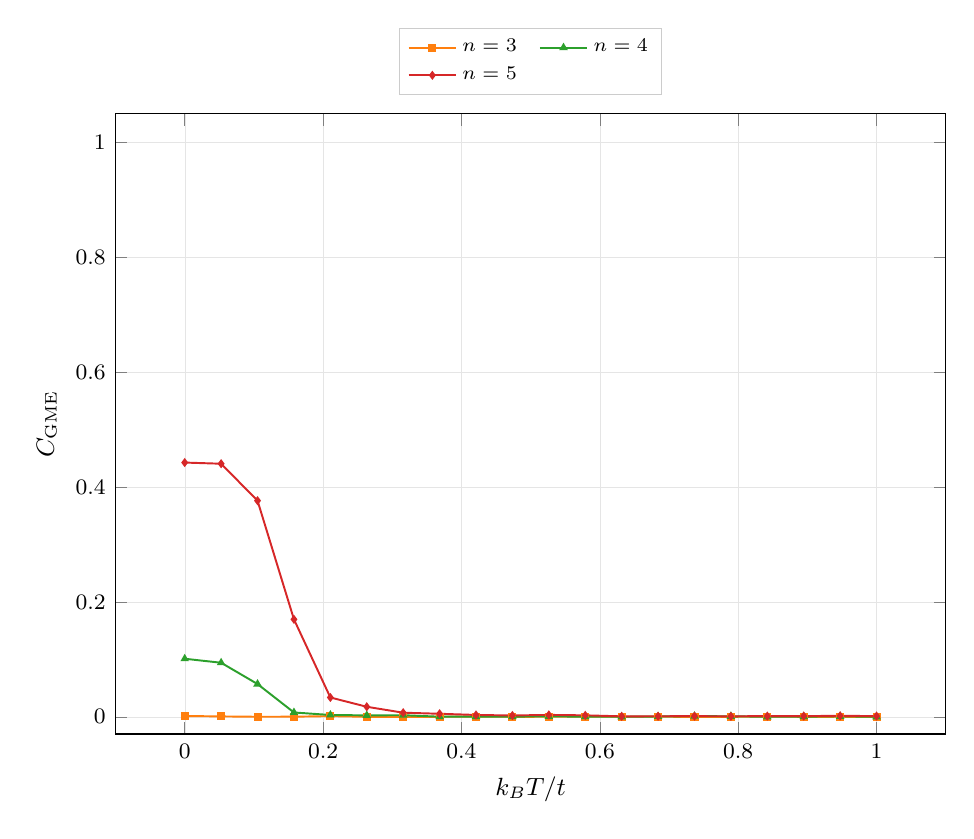
\begin{tikzpicture}
  \begin{axis}[
    width=\columnwidth,
    height=0.78\columnwidth,
    xlabel={$k_B T/t$},
    ylabel={$C_{\mathrm{GME}}$},
    grid=both,
    grid style={line width=.1pt, draw=gray!20},
    tick label style={font=\footnotesize\rmfamily, /pgf/number format/fixed},
    label style={font=\small\rmfamily},
    scaled ticks=false,
    legend style={font=\scriptsize\rmfamily, draw=gray!40, at={(0.5,1.03)}, anchor=south, /tikz/every even column/.append style={column sep=6pt}},
    legend cell align={left},
    legend columns=2,
    ymin=-0.03,
    ymax=1.05,
  ]
    \addplot[color=gmeC1, mark=square*, mark size=1.1pt, line width=0.7pt] coordinates {
        (0,0.001427) (0.052632,0.000672) (0.105263,0.000058) (0.157895,0.000215)
        (0.210526,0.001163) (0.263158,0.000021) (0.315789,0.000001) (0.368421,0.00002)
        (0.421053,0.000484) (0.473684,0.000022) (0.526316,0.000065) (0.578947,0.000253)
        (0.631579,0.000149) (0.684211,0.00008) (0.736842,0.000003) (0.789474,0.000008)
        (0.842105,0.000201) (0.894737,0.000014) (0.947368,0.000055) (1,0)
    };
    \addlegendentry{$n=3$}
    \addplot[color=gmeC2, mark=triangle*, mark size=1.1pt, line width=0.7pt] coordinates {
        (0,0.101118) (0.052632,0.094142) (0.105263,0.057055) (0.157895,0.007555)
        (0.210526,0.003154) (0.263158,0.002518) (0.315789,0.002769) (0.368421,0.00019)
        (0.421053,0.000502) (0.473684,0.000313) (0.526316,0.000808) (0.578947,0.000161)
        (0.631579,0.000035) (0.684211,0.000559) (0.736842,0.001146) (0.789474,0.000957)
        (0.842105,0.000038) (0.894737,0.000299) (0.947368,0.000794) (1,0.000068)
    };
    \addlegendentry{$n=4$}
    \addplot[color=gmeC3, mark=diamond*, mark size=1.1pt, line width=0.7pt] coordinates {
        (0,0.442751) (0.052632,0.440711) (0.105263,0.376353) (0.157895,0.169735)
        (0.210526,0.033663) (0.263158,0.017458) (0.315789,0.007162) (0.368421,0.005285)
        (0.421053,0.003235) (0.473684,0.00229) (0.526316,0.003333) (0.578947,0.002564)
        (0.631579,0.000822) (0.684211,0.00098) (0.736842,0.001129) (0.789474,0.000839)
        (0.842105,0.001255) (0.894737,0.001265) (0.947368,0.00169) (1,0.001271)
    };
    \addlegendentry{$n=5$}
  \end{axis}
\end{tikzpicture}
